% Template example file
% Alvaro Ortiz-Troncoso
% 
% Based on beamer:
% @see https://en.wikibooks.org/wiki/LaTeX/Presentations
% @see http://ctan.127001.ovh/macros/latex/contrib/beamer/doc/beameruserguide.pdf

%%% Local Variables:
%%% mode: latex
%%% TeX-master: t
%%% End:
\documentclass[12pt]{beamer}
\usepackage[utf8]{inputenc}
\usepackage{graphicx}
\usepackage{xcolor}
\usepackage[sfdefault]{roboto}

\definecolor{mfn_green}{HTML}{A1BF23}
\definecolor{mfn_blue}{RGB}{0, 153, 187}

%\renewcommand{\sfdefault}{\roboto}
%\renewcommand{\familydefault}{\sfdefault}

\setbeamercolor{title}{fg=black}
\setbeamerfont{title}{series=\bf,size={\fontsize{25}{30}}}

\setbeamerfont{subtitle}{shape=\itshape,size={\fontsize{20}{25}}}
\setbeamerfont{frametitle}{size={\fontsize{18}{22}}}
\setbeamercolor{frametitle}{fg=black}
\setbeamercolor{footline}{fg=gray}
\beamertemplatenavigationsymbolsempty
%\setbeamertemplate{footline}[page number]
\setbeamertemplate{itemize item}{\color{mfn_green}$\blacktriangleright$}
\setbeamertemplate{caption}{\scriptsize\insertcaption}
\setbeamersize{text margin left=5mm,text margin right=7mm}
\setlength\abovecaptionskip{-5pt}
\setbeamertemplate{footline}{
  \mbox{\hspace{1em}\insertshorttitle}
  \newline\smallskip\newline
  \mbox{\hspace{1em}\insertshortauthor \textbar Museum für Naturkunde Berlin – Leibniz-Institut für Evolutions- und Biodiversitätsforschung}
  \newline\smallskip\newline
}

\title{A presentation example}
\subtitle{Using LaTeX for making presentations}
\author{Alvaro Ortiz-Troncoso}
\date{No particular occasion, 2018}
\subject{Templates and layout}

\begin{document}

%----------------------------------------------------------------------------------------------%
% 0. Title page
{
  \setbeamertemplate{footline}{}
  {
  \logo{
\includegraphics[height=1cm]{mfn_logo_klein.png}\vspace{220pt}}
  \frame{\titlepage}
  }
}
\addtocounter{framenumber}{-1}

% ----------------------------------------------------------------------------------------------%
% 1. A page with a figure
\begin{frame}
  \frametitle{A page with a figure}
  \begin{figure}
    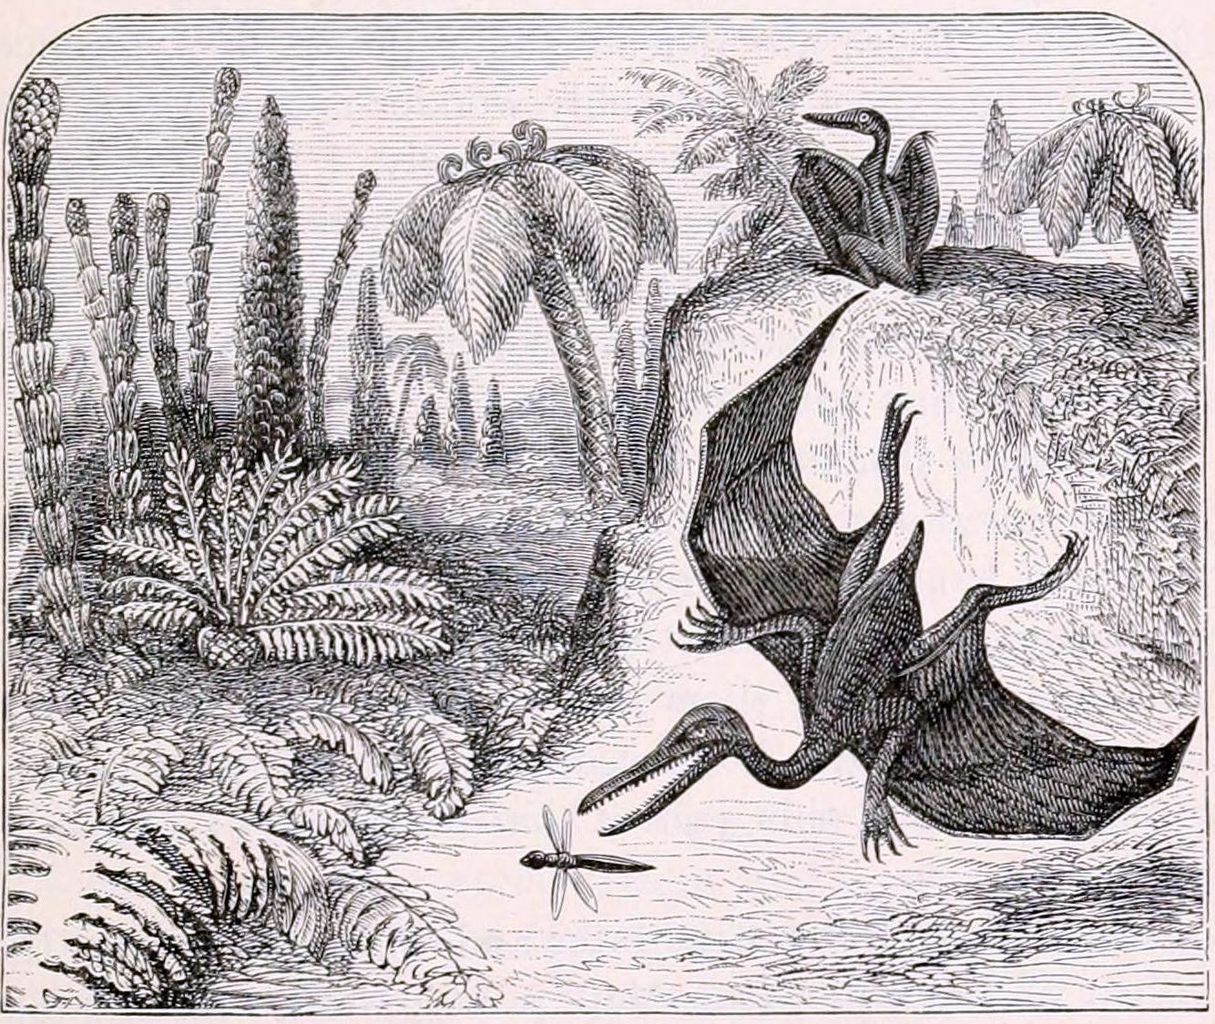
\includegraphics[height=70mm]{Ideal_Landscape_of_a_Prehistoric_Age.jpg}
    \caption{Quackenbos, J.D., 1886. \textit{Illustrated School History of the World}. D. Appleton.}
  \end{figure}
\end{frame}

%----------------------------------------------------------------------------------------------%
% 2. A page with bullets
\begin{frame}
  \frametitle{A page with bullets}
  The cognitive style of PowerPoint is:
  \begin{itemize}
  \item{Over-generalized}
  \item{Imprecise}
  \item{Lightweight}
  \item{Thinly-argued}
  \end{itemize}
  \bigskip
  \begin{center}\scriptsize{Tufte, E.R., 2003. \textit{The cognitive style of PowerPoint}. Cheshire, CT: Graphics Press.}\end{center}  
\end{frame}


% ----------------------------------------------------------------------------------------------%
% 3. A page with a lot of text
{\scriptsize
\begin{frame}
  \frametitle{A page with some text}
Lorem ipsum dolor sit amet, consectetur adipiscing elit, sed do eiusmod tempor incididunt ut labore et dolore magna aliqua. Ut enim ad minim veniam, quis nostrud exercitation ullamco laboris nisi ut aliquip ex ea commodo consequat. Duis aute irure dolor in reprehenderit in voluptate velit esse cillum dolore eu fugiat nulla pariatur. Excepteur sint occaecat cupidatat non proident, sunt in culpa qui officia deserunt mollit anim id est laborum.
\end{frame}
}

% ----------------------------------------------------------------------------------------------%
% 4. A page with even more text
{\scriptsize
\begin{frame}
  \frametitle{A page with more text}
  Alice never could quite make out, in thinking it over afterwards, how it was that they began: all she remembers is, that they were running hand in hand, and the Queen went so fast that it was all she could do to keep up with her: and still the Queen kept crying, ``Faster! Faster!'' but Alice felt she \textit{could not} go faster, though she had no breath left to say so.
  The most curious part of the thing was, that the trees and the other things round them never changed their places at all: however fast they went, they never seemed to pass anything. ``I wonder if all the things move along with us?''\\
    \bigskip
    \textcolor{mfn_green}{Alice konnte, wenn sie später darüber nachdachte, niemals herausbringen, wie sie zu laufen anfingen; sie erinnerte sich nur, daß sie Hand in Hand liefen und daß die Königin so schnell rannte, daß Alice kaum mit ihr Schritt halten konnte; und immer noch rief die Königin: ``Schneller, schneller!'' Aber Alice fühlte, daß sie nicht schneller laufen konnte, obwohl sie nicht genug Atem hatte, um es ihr zu sagen.
      Das Sonderbarste daran war, daß die Bäume und die anderen Gegenstände um sie herum ihre Plätze niemals veränderten. So schnell Alice und die Königin auch liefen, sie schienen niemals an etwas vorbeizulaufen.}\\
  \bigskip
  \scriptsize{Carroll, L., \textit{Through the looking-glass and what Alice found there}. \href{https://en.wikisource.org/wiki/Through_the_Looking-Glass,_and_What_Alice_Found_There/Chapter_II}{\color{mfn_blue}Wikisource} (original text published in 1900)}  
\end{frame}
}

% ----------------------------------------------------------------------------------------------%
% 5. Kontaktdaten
\begin{frame}
  \frametitle{Kontaktdaten / \textcolor{mfn_green}{Contact information}}
  \begin{center}
    \insertauthor \\
    \medskip
    Email: Alvaro.OrtizTroncoso@mfn.berlin \\    
    \medskip
    Web: https://github.com/MfN-Berlin
  \end{center}
\end{frame}

\end{document}


